
\section{"Interaction naturelle" et rehabiliation}
  
\subsection{Applications orientés "fitness"}

\subsubsection{Wii Fit}

Si certaines jeu proposait déjà une interaction naturelle, comme la EyeToy 
de la Playstation de Sony (2003), la console Wii de Nintendo (2006) est 
l'ammorce claire de la
l'enthusiasm présent vis-à-vis de tels interfaces, et cette enthusiasme va bien
au dela des jeux. 
Si nous avons aujourd'hui la Kinect de Microsoft ou encore la
PS Eye de Sony, c'est grâce à son controleur (voir figure~\ref{fig:wii}), 
capable de reconnaître des mouvement à 
travers l'espace grâce à un système d'accéléromètres. 

\begin{figure}[h!]
\centering
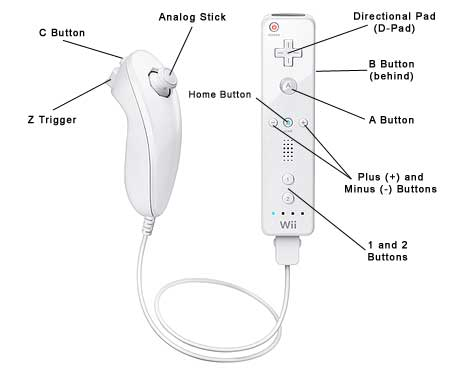
\includegraphics[width=0.7\linewidth]{images/wii_diagram}
\caption{Le controleur de la console Wii de Nintendo.}
\label{fig:wii}
\end{figure}

Avec le jeu Wii Fit Nintendo ajoute la Wii Balance Board (voir figure 
\ref{fig:balance_board}). C'est une accésoire capable de mesurer le 
poids mis sur chaque pied et donc la position du centre de masse. Quant au jeu,
il propose une suivie de la mise en forme du joueur à travers des graphiques, 
points et barres de progress\ref{fig:wii_fit}~: de la "gamification", 
tout simplement.

\begin{figure}[h!]
\centering
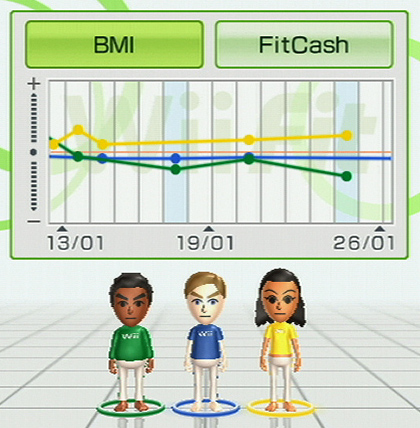
\includegraphics[width=0.5\linewidth]{images/wii_fit}
\caption{Courbes de progression au cours dans temps dans le jeu Wii Fit.}
\label{fig:wii_fit}
\end{figure}

\begin{figure}[h!]
\centering
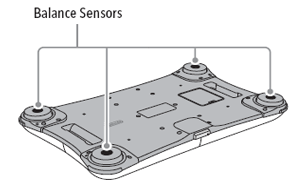
\includegraphics[width=0.5\linewidth]{images/balance_board}
\caption{La Wii Balance board de Nintendo.}
\label{fig:balance_board}
\end{figure}


\subsubsection{Nike+ Kinect Training}


% ------------------------------------------------------------------------------  

\subsection{Applications thérapeutiques}

\subsubsection{"Wiihabilitation"}

Vu que les jeux Wii demandent souvent un mouvement du membre supérieure pour y 
jouer, et de ceux fait de nombreux 
cliniques aux États Unis se sont mis à les détourner pour des buts 
thérapeutiques. Il s'agit bien ici de "détourner"~: rares sont les cas où des
applications spécialistes sont développés pour ce système par un tiers. Ceci
est probablement du à la manque d'outils de développement officiels. Il existe
cependant un très grand nombre d'outils et de bibliothèques non-officiels, et
c'est d'ailleurs le succès de ces efforts qu'a motivé Adafruit à offrir sa prime
pour l'ouverture de la Kinect.
% http://wiibrew.org/wiki/List_of_development_tools



%http://atwiki.assistivetech.net/index.php/Wii_rehab_applications_%28wiihab%29
%http://usatoday30.usatoday.com/tech/science/2008-02-08-wii-rehabilitation_N.htm

\subsubsection{MOJOS}
Lancé en 2010 avec un cycle de développment de 3 ans, 
La Moteur~de~Jeu~Orienté~Santé (MOJOS) est une collaboration entre~:
\begin{itemize}
\item \textbf{professionels} de DIDACT Systèmes, NetDivision et GENIOUS,
\item \textbf{informaticiens} de l'UM2 et du LIRMM,
\item \textbf{médecins} de l'UM1, du CHU et du centre 
de recherche Efficience et Déficience Motrice (EDM),
\item \textbf{l'IDATE}, \emph{think tank} pour l'innovation numérique.
\end{itemize}

\paragraph{}
Son objectif était de développer un moteur jeu permettant 
l'élboration facile d'applications à but thérapeutiques, avec une étude 
expérimentale
par la suite pour vérifier la pertinence de ces applications. En est sorti 
notamment le jeu Voracy Fish de GENIOUS (voir figure~\ref{fig:voracy_fish})
qui propose un exercise du membre supérieur~: le patient contrôle un poisson 
vorace grâce à une Kinect.

\begin{figure}[h!]
\centering
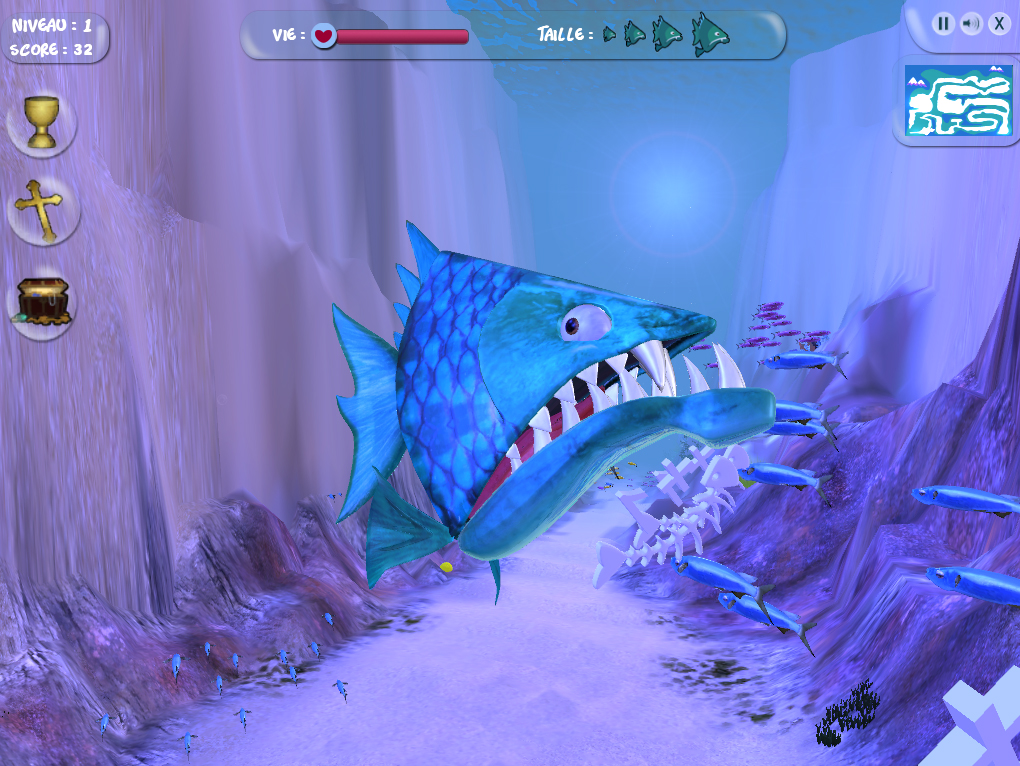
\includegraphics[width=0.8\linewidth]{images/voracy_fish}
\caption{Capture d'écran du jeu "Voracy Fish" de GENIOUS.}
\label{fig:voracy_fish}
\end{figure}

MOJOS se différencie d'un moteur jeu "normale" dans la mesure qu'il propose
un reéquilbrage dynamique de la difficulté à fin de garder le patient dans
ce que Mihály Csíkszentmihályi "Le Flux". Il y a en plus une suivie possible 
des performances du patient par son médecin.
% https://en.wikipedia.org/wiki/Flow_%28psychology%29

% http://www.mojos.fr/home/

\subsubsection{Hammer \& Planks}
Hammer \& Planks, jeu en développement par NaturalPad, se veut à la fois 
ludique et thérapeutique. Il est donc possible de contrôler le jeu par de divers 
modalités dont une manette ou une Kinect.

\begin{figure}[h!]
\centering
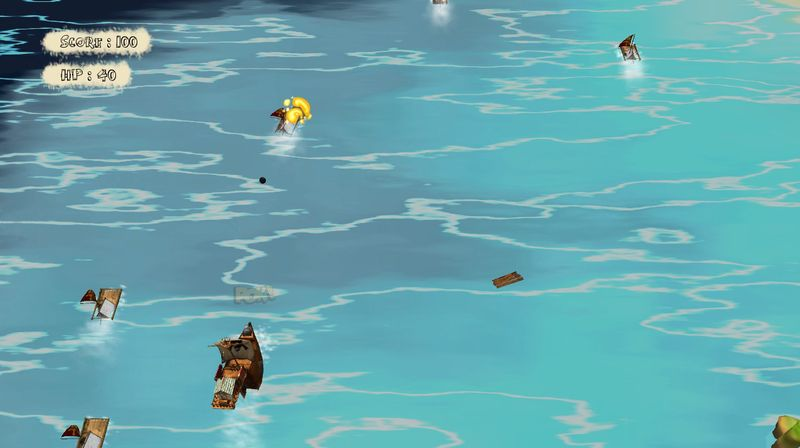
\includegraphics[width=1.0\linewidth]{images/hammer_and_planks}
\caption{Capture d'écran du jeu "Hammer and Planks" de 
NaturalPad.}
\end{figure}

Parmi les points intéressants il est offert ici la possibilité de modifier certains
paramètres du jeu par l'intermédiare d'un terminal annexe, l'idée étant de
permettre à un spécialiste de reéquilbrer le jeu selon les besoins de son
patient.
